\documentclass{beamer}
\usepackage[utf8]{inputenc}
\usepackage{amsmath}
\usepackage{amsfonts}
\usepackage{amssymb}
\usepackage{color}
\usepackage{graphicx}
\usepackage{subfigure}
\usepackage{tabu}
\usepackage{bm}
\usepackage[utf8]{inputenc}
\usepackage[english]{babel}
\usepackage{minted}
\usepackage{siunitx}

%Full justify
\renewcommand{\raggedright}{\leftskip=0pt \rightskip=0pt plus 0cm}
\raggedright

\title{Automatic Parking Using Reinforcement Learning}
\author{Tao Chen}
\institute[Shanghai Lingxian]
{
  Shanghai LingXian Robotics
}


\date{Nov 29, 2016}
\subject{Automatic Parking Using Reinforcement Learning}

\AtBeginSection[]
{
  \begin{frame}<beamer>{Outline}
    \tableofcontents[currentsection]
  \end{frame}
}

\setbeamertemplate{footline}[frame number]
\begin{document}
\begin{frame}
  \titlepage
\end{frame}

\begin{frame}{Outline}
  \tableofcontents
\end{frame}

\section{Working Principle}

\begin{frame}{Reinforcement Learning Framework}
\begin{figure}
    \centering
    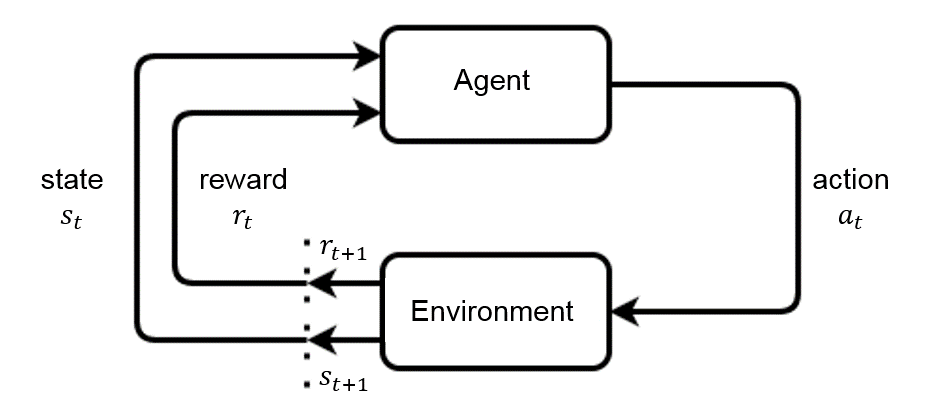
\includegraphics[width=10cm]{agent_env.png}
    \caption{Reinforcement Learning Framework}
    \label{fig:Reinforcement Learning Framework}
\end{figure}    
\end{frame}


\begin{frame}{Q-Learning}
\begin{itemize}
\item{What is Q-Learning?}
\begin{itemize}
\item{A model-free reinfocement learning technique}
\item{Work by learning an {\color{blue}action-value function} that ultimately gives the {\color{blue}expected utility} of taking a given action in a given state and following the optimal policy thereafter}
\item{The utility function tells how good an action is given a certain state}
\item{An optimal policy selects an action with the highest utility value in each state}
\end{itemize}
\end{itemize}
Q-learning has been proven to {\color{blue}converge} to the {\color{blue}optimum action-values} so long as all actions are repeatedly sampled in all states and the action-values are represented discretely.
\end{frame}


\begin{frame}{Q-Learning Algorithm}
\begin{itemize}
\item{Initialize Q-values ($Q(s,a)$) arbitrarily for all state-action pairs}
\item{While not stopped:}
\begin{itemize}
\item{Choose an action $\boldsymbol{a}$ in the current state $\boldsymbol{s}$ based on current Q-value estimates ($\bm{Q(s,*)}$)}
\item{Execute the action $\boldsymbol{a}$, receive immdediate reward $\bm{r}$, observe the outcome state $\bm{s^\prime}$}
\item{Update the table entry for $\bm{Q(s,a)}$: \\
$$Q(s,a) = Q(s,a) + \alpha[r + \gamma\underset{a^\prime}{max}Q(s^\prime, a^\prime) - Q(s,a)] $$ }
\item{$\bm{s} = \bm{s^\prime}$}
\end{itemize}
\item{Remark: $\alpha$: learning rate, $\gamma$: discount factor} 
\end{itemize}
\end{frame}



\begin{frame}{Exploration and Exploitation}
\begin{itemize}
\item{\textbf{\color{blue}Exploitation:} make best decision given current information}
\begin{itemize}
\item{short-term, immediate, certain benefits}
\end{itemize}
\item{\textbf{\color{blue}Exploration:} gather more information}
\begin{itemize}
\item{long-term, risky, uncertain}
\end{itemize}
\item{\textbf{All Exploitation:} locked-in to suboptimal equilibria (local maxima), cannot adapt to changing circumstances }
\item{\textbf{All Exploration:} costs of experimentation without any of its benefits}
\item{The best \textbf{long-term strategy} may involve \textbf{short-term sacrifies}}
\item{Gather \textbf{enough information} to make the best overall decisions}
\end{itemize}
\end{frame}


\begin{frame}{$\epsilon$-greedy algorithm}
\begin{itemize}
\item{Greedy Algorithm: an algorithm that always takes whatever action seems best at the present moment}
\item{Epsilon Greedy Algorithm: an algorithm that generally exploits the best available option, but has probability $\epsilon$ to randomly explore action space}
\end{itemize}

\[ a = 
  \begin{cases}
  \underset{a}{argmax}(Q(s,*)) & \quad \text{with probability } 1 - \epsilon \\
  random\ action & \quad \text{with probability } \epsilon \\
  \end{cases}
\]
\end{frame}


\begin{frame}{Q-Learning Parameters}
\begin{itemize}
\item{\textbf{Learning rate $\alpha$:} determine to what extent the newly acquired information will override the old information}
\begin{itemize}
\item{0: make the agent not learn anything}
\item{1: make the agent consider only the most recent information}
\end{itemize}
\item{\textbf{Discount factor $\gamma$:} determine importance of future rewards}
\begin{itemize}
\item{0: make the agent short-sighted by only considering current rewards}
\item{1: make the agent strive for a long-term high reward}
\end{itemize}
\end{itemize}
\end{frame}

\section{Source Code}

\begin{frame}[fragile]{Auomatic Parking Agent Source Code}
\usemintedstyle{colorful}
\tiny{
\begin{minted}{python}
    def update(self):
        agent_pose = self.env.sense()
        self.state = states(x = agent_pose[0], y = agent_pose[1], theta = agent_pose[2])

        step = self.env.get_steps()
        if self.env.enforce_deadline:
            deadline = self.env.get_deadline()

        # Select action according to the policy
        action, max_q_value = self.get_action(self.state)

        # Execute action and get reward
        next_agent_pose,reward = self.env.act(self, action)

        # Learn policy based on state, action, reward
        if not self.test:
            if self.prev_action != None:
                    self.update_q_values(self.prev_state, self.prev_action, 
                                         self.prev_reward, max_q_value)

            if self.env.enforce_deadline:
                print "LearningAgent.update(): step = {}, deadline = {},
                       state = {}, action = {}, reward = {}".format(step, deadline,self.state,
                       action, reward)
            else:
                print "LearningAgent.update(): step = {}, state = {}, 
                       action = {}, reward = {}".format(step, self.state, action, reward)

        self.save_state(self.state, action, reward)

\end{minted}
}
\end{frame}


\begin{frame}[fragile]{Auomatic Parking Agent Source Code}
\usemintedstyle{colorful}
\tiny{
\begin{minted}{python}
    def update_q_values(self, prev_state, prev_action, prev_reward, max_q_value):
        old_q_value = self.Q_values.get((prev_state, prev_action), self.default_q)
        new_q_value = old_q_value + self.learning_rate * (prev_reward + self.gamma * max_q_value 
                      - old_q_value)
        self.Q_values[(prev_state, prev_action)] = new_q_value




    def get_maximum_q_value(self, state):
        q_value_selected = -10000000
        for action in car_sim_env.valid_actions:
            q_value = self.get_q_value(state, action)
            if q_value > q_value_selected:
                q_value_selected = q_value
                action_selected = action
            elif q_value == q_value_selected: 
            # if there are two actions that lead to same q value, 
            # we need to randomly choose one between them
                action_selected = random.choice([action_selected, action])
        return action_selected, q_value_selected
       

\end{minted}
}
\end{frame}




\begin{frame}[fragile]{Auomatic Parking Agent Source Code}
\usemintedstyle{colorful}
\tiny{
\begin{minted}{python}
    def get_action(self, state):
        if random.random() < self.epsilon:
            action_selected = random.choice(car_sim_env.valid_actions)
            q_value_selected = self.get_q_value(state, action_selected)
        else:
            action_selected, q_value_selected = self.get_maximum_q_value(state)
        return action_selected, q_value_selected





    def get_q_value(self, state, action):
        return self.Q_values.get((state,action), self.default_q)
\end{minted}
}
\end{frame}


\begin{frame}[fragile]{Auomatic Parking Environment Source Code}
\usemintedstyle{colorful}
\tiny{
\begin{minted}{python}
    def sense(self):
        agent_pose = np.zeros(3) #[x, y, theta]
        agent_pose[0] = self.agent_pos[0]
        agent_pose[1] = self.agent_pos[1]
        agent_pose[2] = np.arctan2(self.agent_ori[2], self.agent_ori[3]) * 2
        agent_pose[2] = (agent_pose[2] + 2 * np.pi) % (2 * np.pi)
        agent_pose[0] = np.floor((np.floor(agent_pose[0] / (self.grid_width / 2)) + 1) / 2) *
                        self.grid_width
        agent_pose[1] = np.floor((np.floor(agent_pose[1] / (self.grid_width / 2)) + 1) / 2) * 
                        self.grid_width
        idx = np.floor(agent_pose[2] / (self.angle_blockwidth / 2))
        if idx % 2 == 0:
            idx = idx / 2
        else:
            idx = (idx + 1) / 2
        agent_pose[2] = idx % 16
        # agent_pose[2] represents the region the car's angle belongs to
        # [-11.25, 11.25) is region 0
        # [11.25, 33.75) is region 1
        # ...
        # [-33.75, -11.25) is region 15
        return agent_pose
\end{minted}
}
\end{frame}

\begin{frame}[fragile]{Auomatic Parking Environment Source Code}
\usemintedstyle{colorful}
\tiny{
\begin{minted}{python}
    def reset(self):
        self.done = False
        self.t = 0

        x, y, z, theta = self.generate_agent_pose()
        self.reset_world(x,y,theta)
        if self.enforce_deadline:
            self.deadline = self.cal_deadline(x, y)
        print '   agent starting pose:', x, y, theta
\end{minted}
}
\end{frame}


\begin{frame}[fragile]{Auomatic Parking Environment Source Code}
\usemintedstyle{colorful}
\tiny{
\begin{minted}{python}
    def step(self):
        # Update agent
        self.agent.update()

        if self.done:
            return

        if self.agent is not None:
            if self.t >= self.hard_time_limit:
                print "Environment.step(): Primary agent hit hard time limit! Trial aborted."
                self.done = True
                self.num_hit_time_limit += 1

            elif self.enforce_deadline and self.t >= self.deadline:
                print "Environment.step(): Primary agent ran out of time! Trial aborted."
                self.done = True
                self.num_out_of_time += 1

            self.t += 1
\end{minted}
}
\end{frame}


\begin{frame}[fragile]{Auomatic Parking Environment Source Code}
\usemintedstyle{colorful}
\tiny{
\begin{minted}{python}
    def act(self, agent, action):
        self.set_agent_velocity(self.valid_actions_dict[action])
        tiem.sleep(self.step_length / self.speed)
        self.set_agent_velocity(np.array([0,0]))
        reward = 0.0

        agent_pose = self.sense()

        if self.hit_wall_check(agent_pose):
            self.hit_wall_times += 1
            self.done = True
            reward = -20.0

        elif self.reach_terminal(agent_pose):
            if self.t < self.hard_time_limit and self.t < self.deadline:
                reward = 40.0
                self.done = True
                self.succ_times += 1
                print '----------------------------------------------------------------------'
                print '----------------------------------------------------------------------'
                print '----------------------------------------------------------------------'
                print '----------------------------------------------------------------------'
                print "Environment.act(): Agent has reached destination!"


        elif self.fixed_car_movement_check():
            self.hit_car_times += 1
            self.done = True
            reward = -5.0

        return agent_pose, reward
\end{minted}
}
\end{frame}

\section{Training}

\begin{frame}{Training Stages}
\begin{itemize}
\item{Training is separated into three stages:}
\begin{itemize}
\item{stage one: far region to close region}
\item{stage two: close region to region adjacent to fixed car}
\item{stage three: region adjacent to fixed car to terminal}
\end{itemize}
\end{itemize}
\end{frame}

\begin{frame}{Stage One}
	\begin{figure}
		\centering
		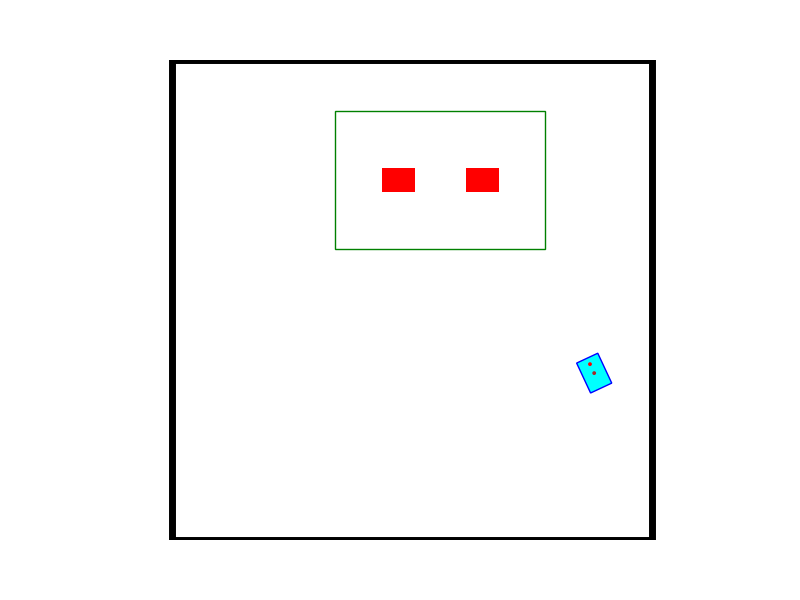
\includegraphics[width=8cm]{stage_one_sim.png}
		\caption{Stage One}
		\label{fig:Stage One}
	\end{figure}
\end{frame}

\begin{frame}{Stage Two}
	\begin{figure}
		\centering
		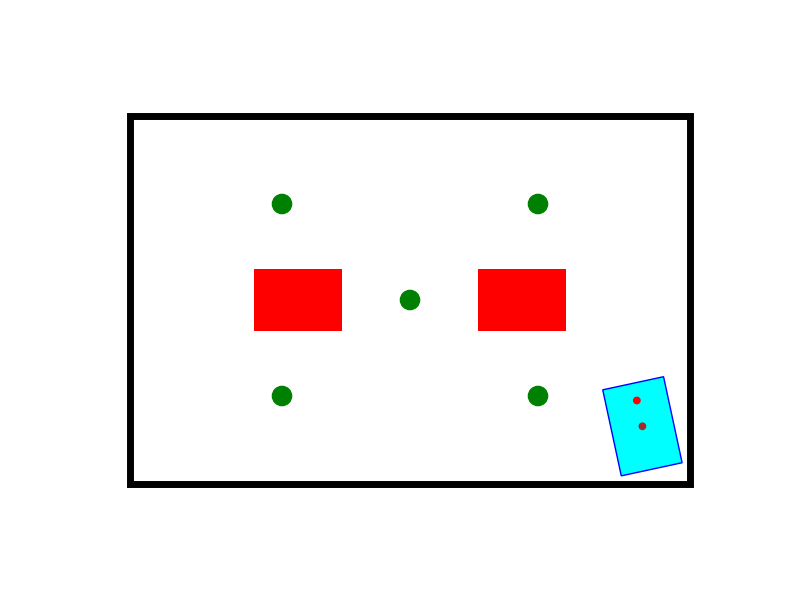
\includegraphics[width=8cm]{stage_two_sim.png}
		\caption{Stage Two}
		\label{fig:Stage Two}
	\end{figure}
\end{frame}

\begin{frame}{Stage Three}
\begin{figure}
    \centering
    \begin{minipage}{4cm}
    	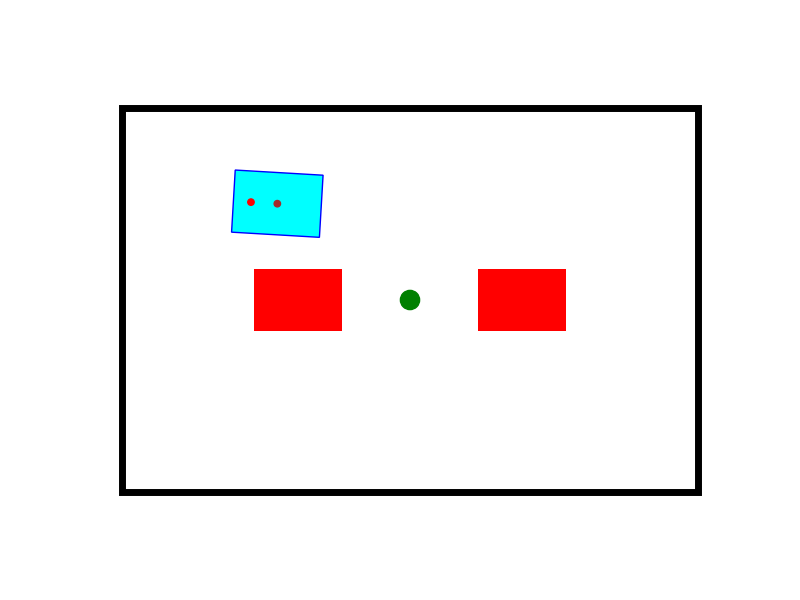
\includegraphics[width=4cm]{top_left_sim.png}
    \end{minipage}
    \begin{minipage}{4cm}
    	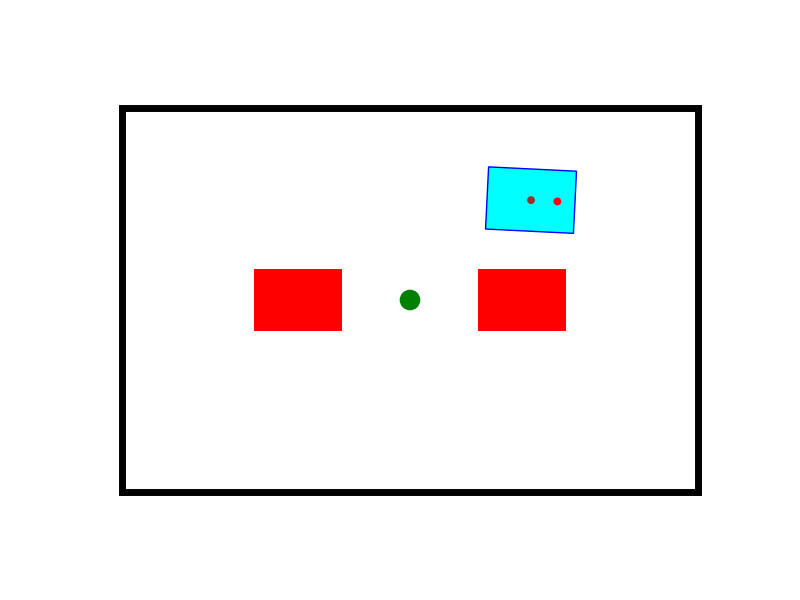
\includegraphics[width=4cm]{top_right_sim.png}
    \end{minipage}
    
    \begin{minipage}{4cm}
    	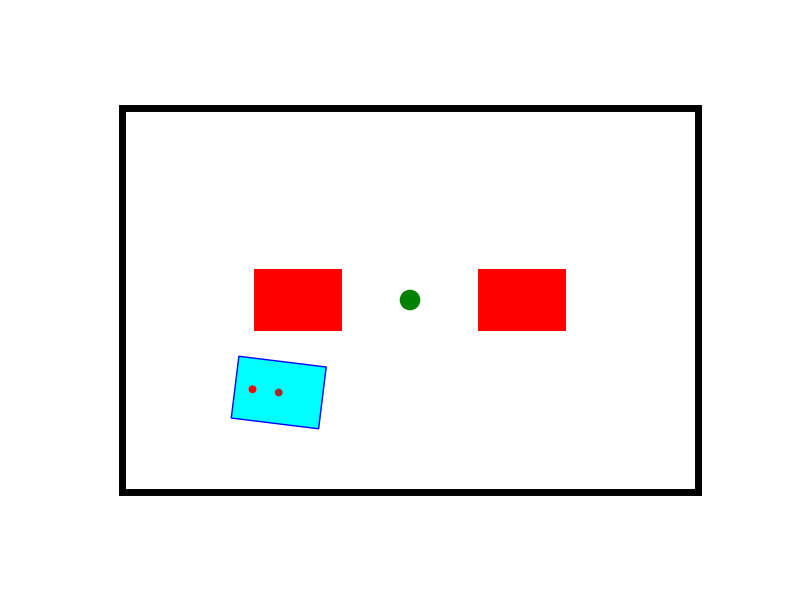
\includegraphics[width=4cm]{bottom_left_sim.png}
    \end{minipage}
    \begin{minipage}{4cm}
    	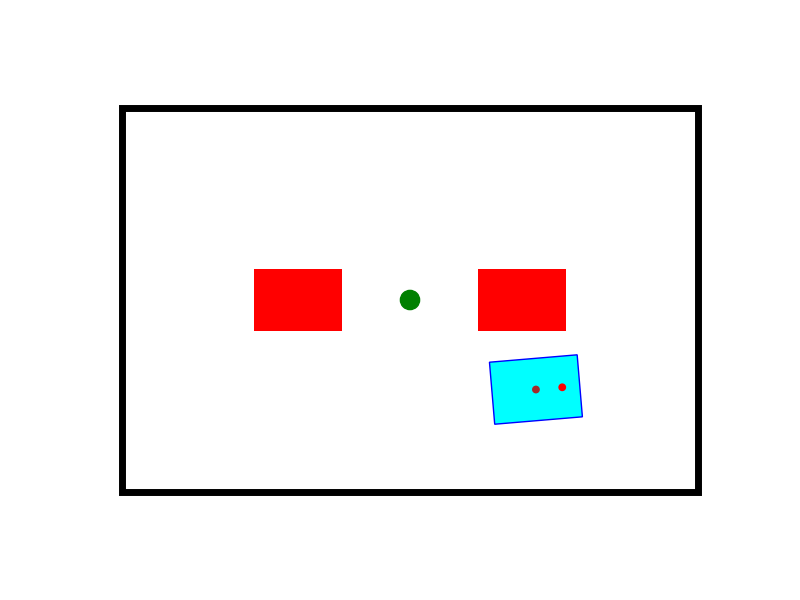
\includegraphics[width=4cm]{bottom_right_sim.png}
    \end{minipage}
    
    \caption{TOP LEFT, TOP RIGHT,
        	BOTTOM LEFT, BOTTOM RIGHT}
\end{figure} 
\end{frame}

\begin{frame}{Stage One Training}
\begin{figure}
    \centering
    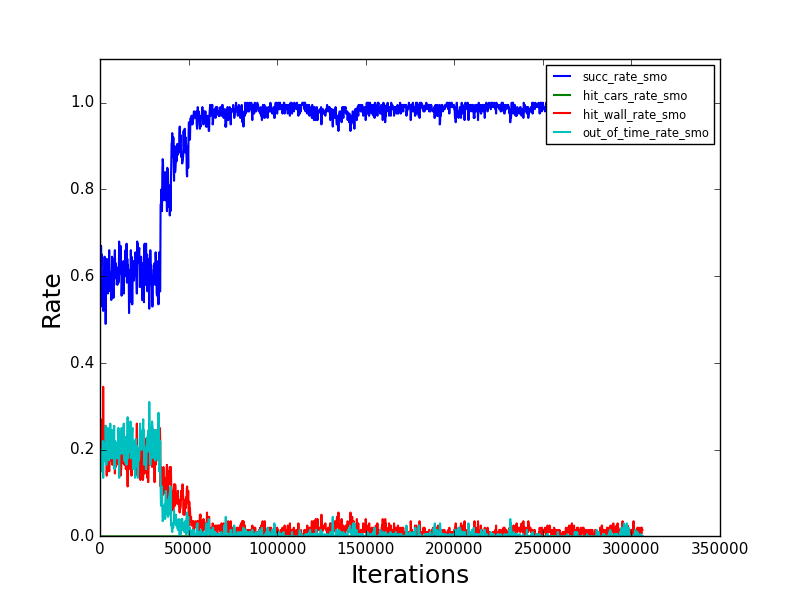
\includegraphics[width=10cm]{stage_one.png}
    \caption{Stage One Training}
    \label{fig:Stage One Training}
\end{figure} 
\end{frame}

\begin{frame}{Stage Two Training}
\begin{figure}
    \centering
    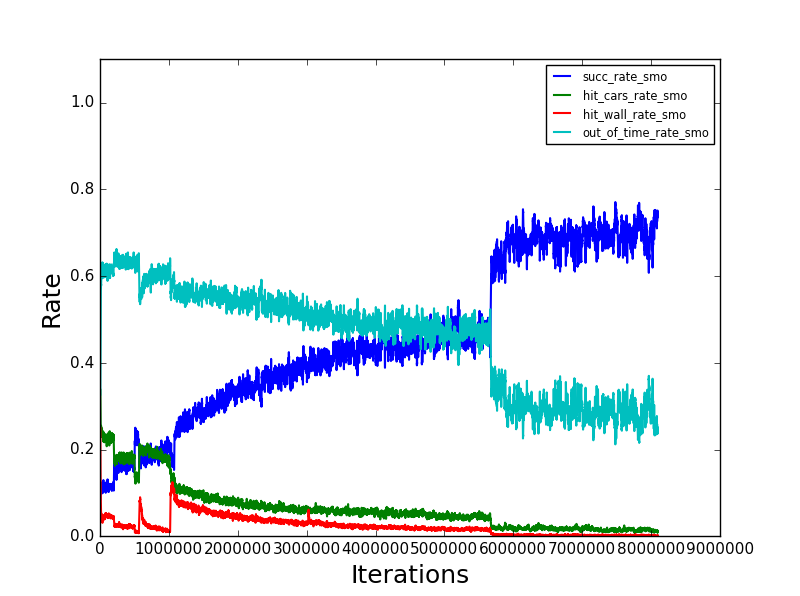
\includegraphics[width=10cm]{stage_two.png}
    \caption{Stage Two Training}
    \label{fig:Stage Two Training}
\end{figure} 
\end{frame}

\begin{frame}{Stage Three Training}
\begin{figure}
    \centering
    \begin{minipage}{4.5cm}
    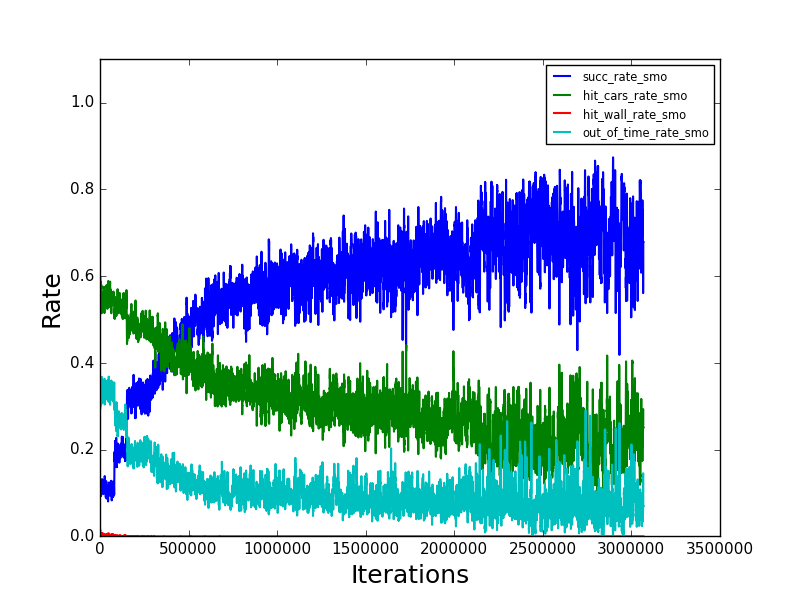
\includegraphics[width=4.5cm]{top_left.png}
    \end{minipage}
    \begin{minipage}{4.5cm}
    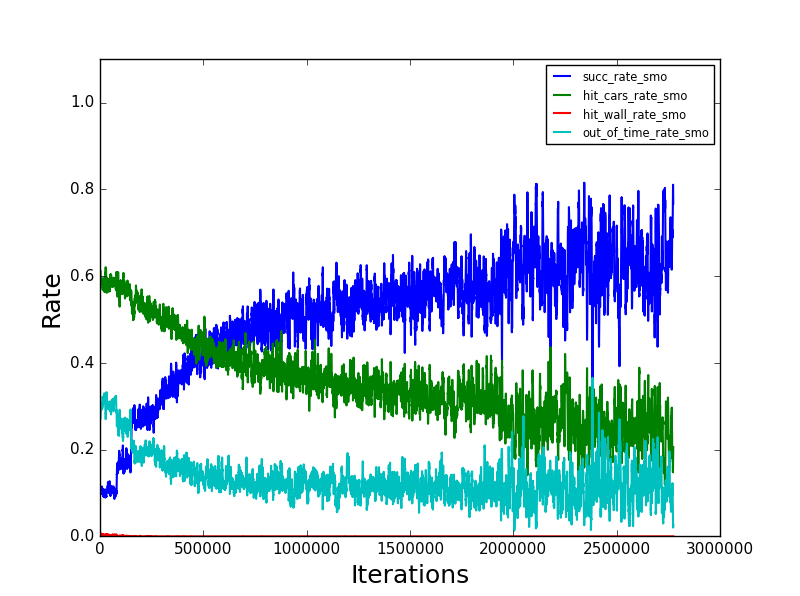
\includegraphics[width=4.5cm]{top_right.png}
    \end{minipage}
    
    \begin{minipage}{4.5cm}
    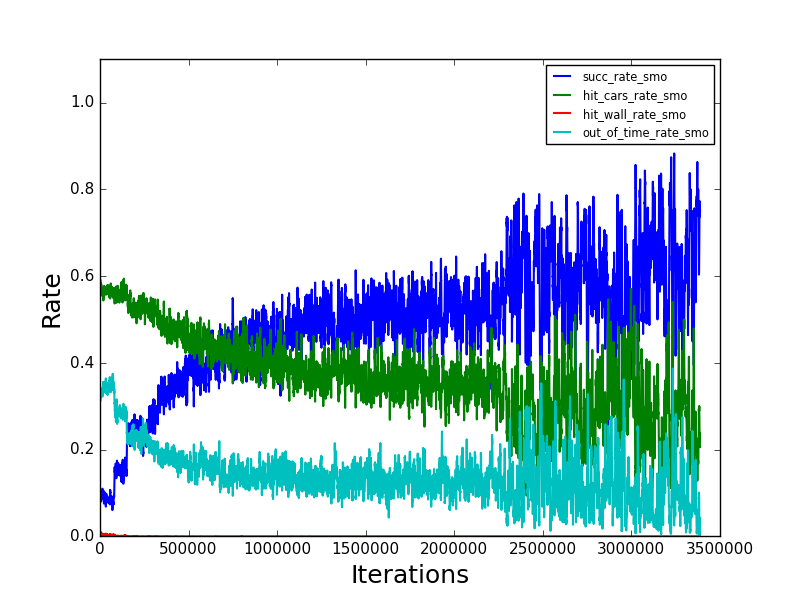
\includegraphics[width=4.5cm]{bottom_left.png}
    \end{minipage}
    \begin{minipage}{4.5cm}
    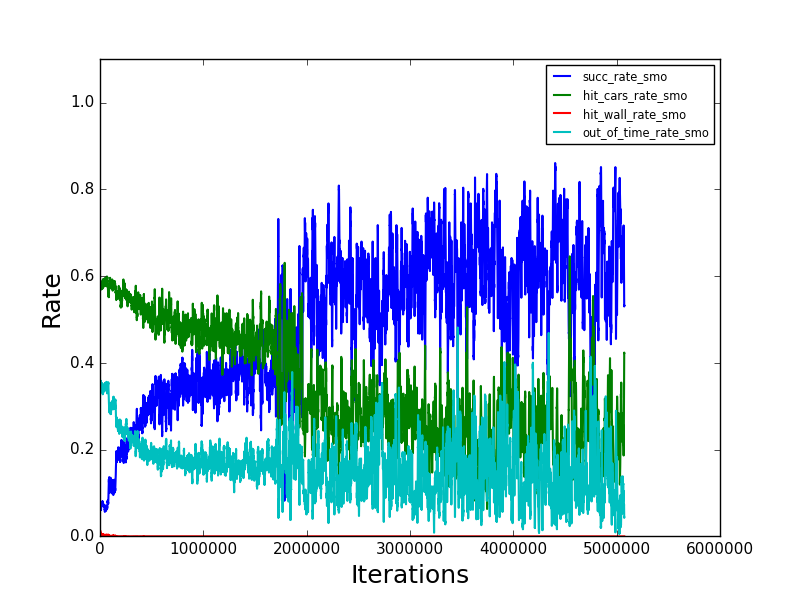
\includegraphics[width=4.5cm]{bottom_right.png}
    \end{minipage}
    \caption{TOP LEFT, TOP RIGHT,
             BOTTOM LEFT, BOTTOM RIGHT}
\end{figure} 
\end{frame}


\begin{frame}{Combining Three Stages}
\begin{figure}
    \centering
    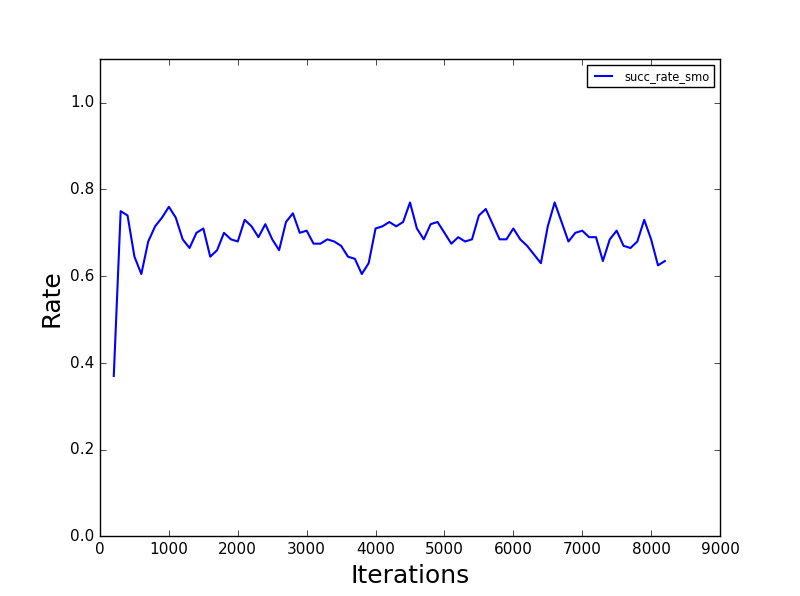
\includegraphics[width=10cm]{whole_sim.png}
    \caption{Combining Three Stages}
    \label{fig:Combining Three Stages}
\end{figure}
\end{frame}

\begin{frame}{Effect of $\epsilon$}
\begin{figure}
    \centering
    \begin{minipage}{5cm}
    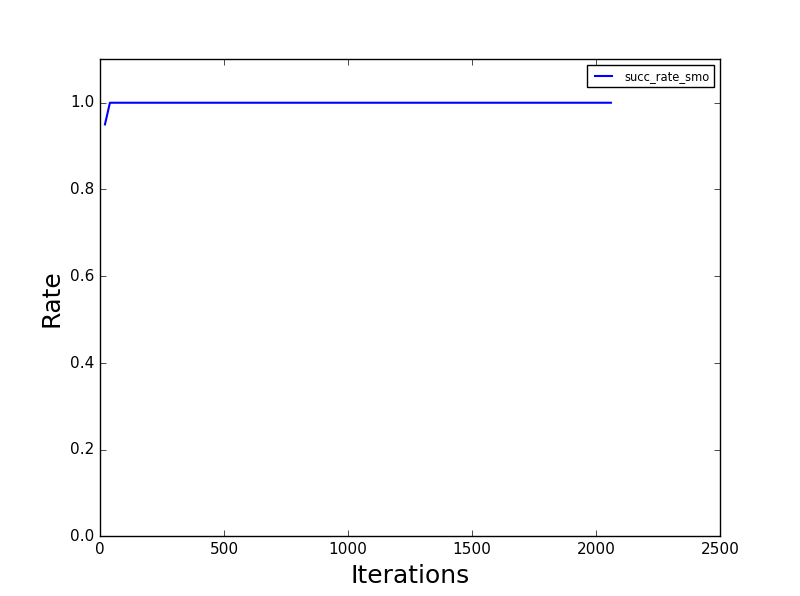
\includegraphics[width=5cm]{0.png}
    \caption{$\epsilon = 0$}
    \end{minipage}
    \begin{minipage}{5cm}
    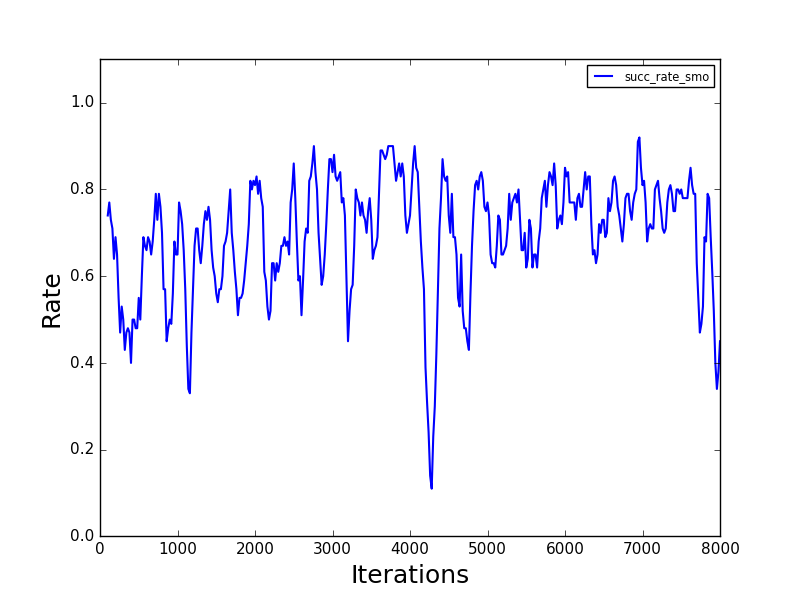
\includegraphics[width=5cm]{0_05.png}
    \caption{$\epsilon = 0.05$}
    \end{minipage}
\end{figure} 
\end{frame}


\begin{frame}{Effect of $\epsilon$}
\begin{figure}
    \centering
    \begin{minipage}{5cm}
    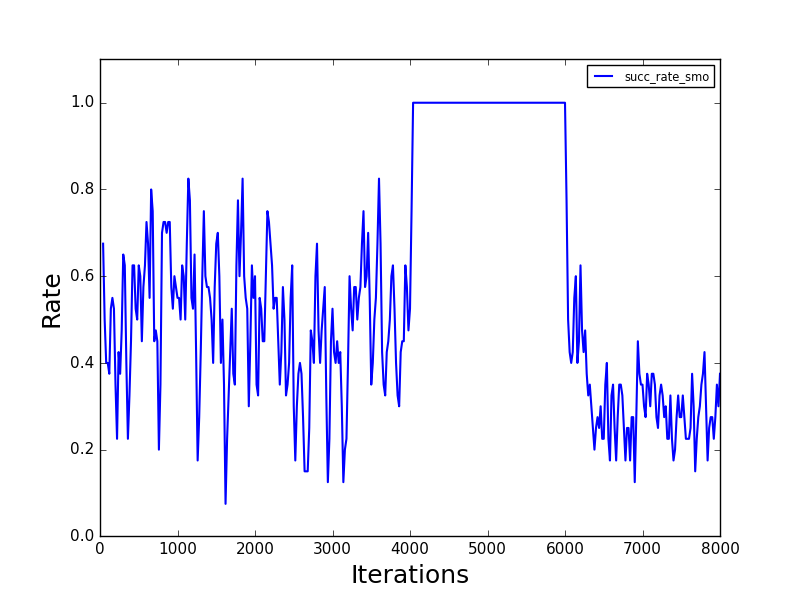
\includegraphics[width=5cm]{0_1_vari_theta.png}
    \caption{$\epsilon = 0.1$}
    \end{minipage}
    \begin{minipage}{5cm}
    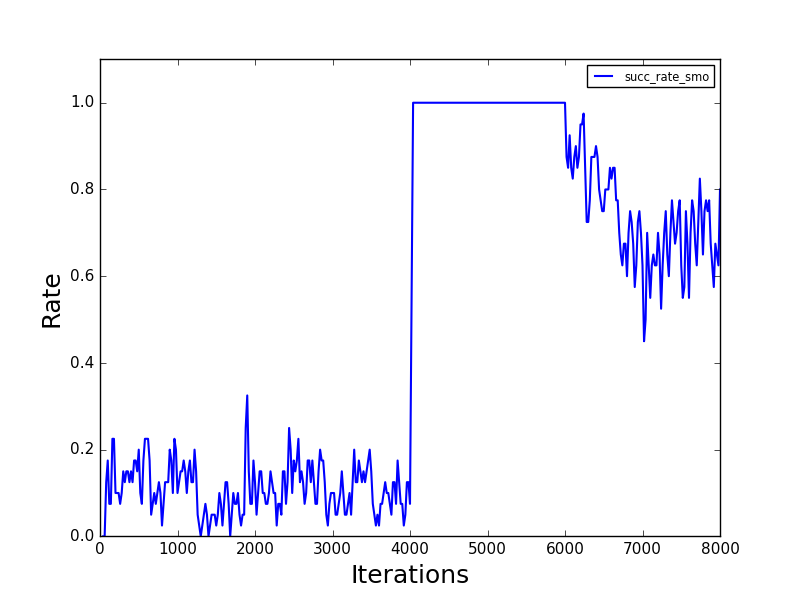
\includegraphics[width=5cm]{0_4_vari_theta.png}
    \caption{$\epsilon = 0.4$}
    \end{minipage}
\end{figure} 

\footnotesize{
Procedure:
\begin{itemize}
	\item {use the $\epsilon$ specified above to train the agent starting from top left region to the terminal for 4000 episodes}
	\item {test the agent with $\epsilon = 0$ for 2000 episodes}
	\item {add noise to the agent's initial angle ($\pm11.25\si{\degree}$ for 2000 episodes)}
\end{itemize}

}

\end{frame}



\end{document}